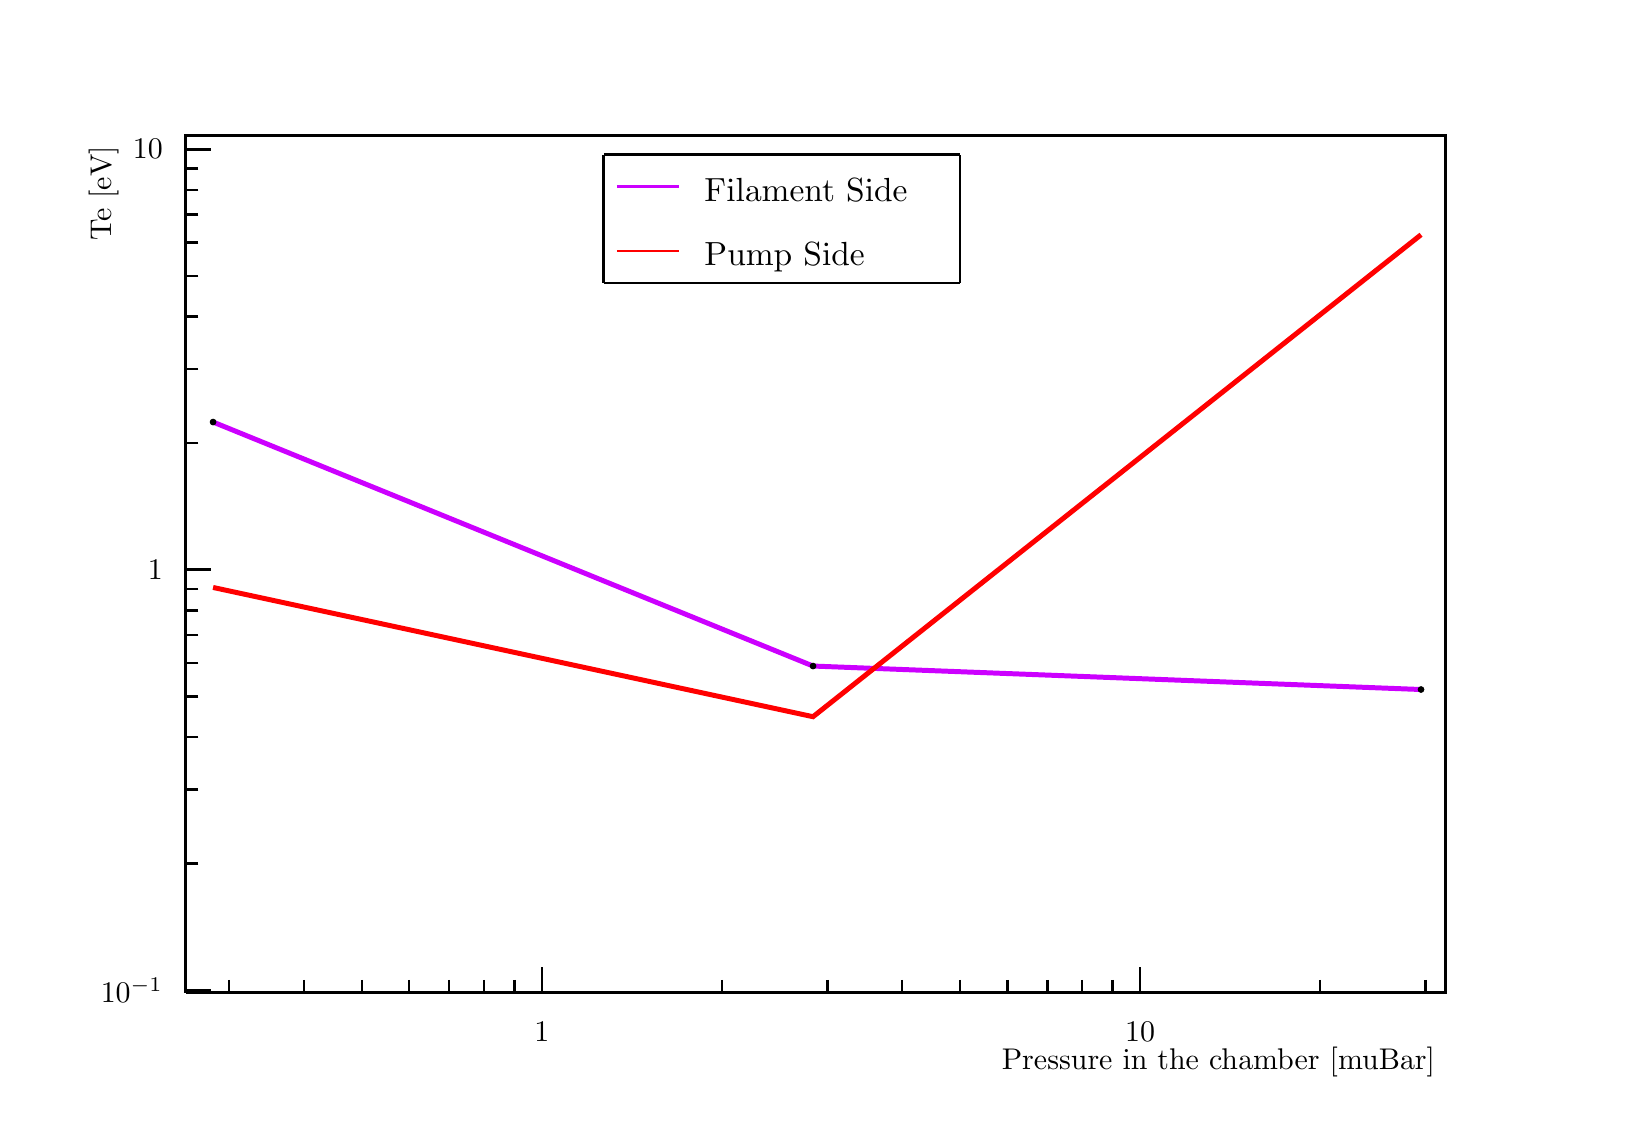
\begin{tikzpicture}
\pgfdeclareplotmark{cross} {
\pgfpathmoveto{\pgfpoint{-0.3\pgfplotmarksize}{\pgfplotmarksize}}
\pgfpathlineto{\pgfpoint{+0.3\pgfplotmarksize}{\pgfplotmarksize}}
\pgfpathlineto{\pgfpoint{+0.3\pgfplotmarksize}{0.3\pgfplotmarksize}}
\pgfpathlineto{\pgfpoint{+1\pgfplotmarksize}{0.3\pgfplotmarksize}}
\pgfpathlineto{\pgfpoint{+1\pgfplotmarksize}{-0.3\pgfplotmarksize}}
\pgfpathlineto{\pgfpoint{+0.3\pgfplotmarksize}{-0.3\pgfplotmarksize}}
\pgfpathlineto{\pgfpoint{+0.3\pgfplotmarksize}{-1.\pgfplotmarksize}}
\pgfpathlineto{\pgfpoint{-0.3\pgfplotmarksize}{-1.\pgfplotmarksize}}
\pgfpathlineto{\pgfpoint{-0.3\pgfplotmarksize}{-0.3\pgfplotmarksize}}
\pgfpathlineto{\pgfpoint{-1.\pgfplotmarksize}{-0.3\pgfplotmarksize}}
\pgfpathlineto{\pgfpoint{-1.\pgfplotmarksize}{0.3\pgfplotmarksize}}
\pgfpathlineto{\pgfpoint{-0.3\pgfplotmarksize}{0.3\pgfplotmarksize}}
\pgfpathclose
\pgfusepathqstroke
}
\pgfdeclareplotmark{cross*} {
\pgfpathmoveto{\pgfpoint{-0.3\pgfplotmarksize}{\pgfplotmarksize}}
\pgfpathlineto{\pgfpoint{+0.3\pgfplotmarksize}{\pgfplotmarksize}}
\pgfpathlineto{\pgfpoint{+0.3\pgfplotmarksize}{0.3\pgfplotmarksize}}
\pgfpathlineto{\pgfpoint{+1\pgfplotmarksize}{0.3\pgfplotmarksize}}
\pgfpathlineto{\pgfpoint{+1\pgfplotmarksize}{-0.3\pgfplotmarksize}}
\pgfpathlineto{\pgfpoint{+0.3\pgfplotmarksize}{-0.3\pgfplotmarksize}}
\pgfpathlineto{\pgfpoint{+0.3\pgfplotmarksize}{-1.\pgfplotmarksize}}
\pgfpathlineto{\pgfpoint{-0.3\pgfplotmarksize}{-1.\pgfplotmarksize}}
\pgfpathlineto{\pgfpoint{-0.3\pgfplotmarksize}{-0.3\pgfplotmarksize}}
\pgfpathlineto{\pgfpoint{-1.\pgfplotmarksize}{-0.3\pgfplotmarksize}}
\pgfpathlineto{\pgfpoint{-1.\pgfplotmarksize}{0.3\pgfplotmarksize}}
\pgfpathlineto{\pgfpoint{-0.3\pgfplotmarksize}{0.3\pgfplotmarksize}}
\pgfpathclose
\pgfusepathqfillstroke
}
\pgfdeclareplotmark{newstar} {
\pgfpathmoveto{\pgfqpoint{0pt}{\pgfplotmarksize}}
\pgfpathlineto{\pgfqpointpolar{44}{0.5\pgfplotmarksize}}
\pgfpathlineto{\pgfqpointpolar{18}{\pgfplotmarksize}}
\pgfpathlineto{\pgfqpointpolar{-20}{0.5\pgfplotmarksize}}
\pgfpathlineto{\pgfqpointpolar{-54}{\pgfplotmarksize}}
\pgfpathlineto{\pgfqpointpolar{-90}{0.5\pgfplotmarksize}}
\pgfpathlineto{\pgfqpointpolar{234}{\pgfplotmarksize}}
\pgfpathlineto{\pgfqpointpolar{198}{0.5\pgfplotmarksize}}
\pgfpathlineto{\pgfqpointpolar{162}{\pgfplotmarksize}}
\pgfpathlineto{\pgfqpointpolar{134}{0.5\pgfplotmarksize}}
\pgfpathclose
\pgfusepathqstroke
}
\pgfdeclareplotmark{newstar*} {
\pgfpathmoveto{\pgfqpoint{0pt}{\pgfplotmarksize}}
\pgfpathlineto{\pgfqpointpolar{44}{0.5\pgfplotmarksize}}
\pgfpathlineto{\pgfqpointpolar{18}{\pgfplotmarksize}}
\pgfpathlineto{\pgfqpointpolar{-20}{0.5\pgfplotmarksize}}
\pgfpathlineto{\pgfqpointpolar{-54}{\pgfplotmarksize}}
\pgfpathlineto{\pgfqpointpolar{-90}{0.5\pgfplotmarksize}}
\pgfpathlineto{\pgfqpointpolar{234}{\pgfplotmarksize}}
\pgfpathlineto{\pgfqpointpolar{198}{0.5\pgfplotmarksize}}
\pgfpathlineto{\pgfqpointpolar{162}{\pgfplotmarksize}}
\pgfpathlineto{\pgfqpointpolar{134}{0.5\pgfplotmarksize}}
\pgfpathclose
\pgfusepathqfillstroke
}
\definecolor{c}{rgb}{1,1,1};
\draw [color=c, fill=c] (0,0) rectangle (20,13.6103);
\draw [color=c, fill=c] (2,1.36103) rectangle (18,12.2493);
\definecolor{c}{rgb}{0,0,0};
\draw [c,line width=0.9] (2,1.36103) -- (2,12.2493) -- (18,12.2493) -- (18,1.36103) -- (2,1.36103);
\definecolor{c}{rgb}{1,1,1};
\draw [color=c, fill=c] (2,1.36103) rectangle (18,12.2493);
\definecolor{c}{rgb}{0,0,0};
\draw [c,line width=0.9] (2,1.36103) -- (2,12.2493) -- (18,12.2493) -- (18,1.36103) -- (2,1.36103);
\draw [c,line width=0.9] (2,1.36103) -- (18,1.36103);
\draw [c,line width=0.9] (2.55171,1.52436) -- (2.55171,1.36103);
\draw [c,line width=0.9] (3.50076,1.52436) -- (3.50076,1.36103);
\draw [c,line width=0.9] (4.23689,1.52436) -- (4.23689,1.36103);
\draw [c,line width=0.9] (4.83836,1.52436) -- (4.83836,1.36103);
\draw [c,line width=0.9] (5.34689,1.52436) -- (5.34689,1.36103);
\draw [c,line width=0.9] (5.78741,1.52436) -- (5.78741,1.36103);
\draw [c,line width=0.9] (6.17597,1.52436) -- (6.17597,1.36103);
\draw [c,line width=0.9] (6.52354,1.68768) -- (6.52354,1.36103);
\draw [anchor=base] (6.52354,0.745165) node[scale=1.08185, color=c, rotate=0]{1};
\draw [c,line width=0.9] (8.81019,1.52436) -- (8.81019,1.36103);
\draw [c,line width=0.9] (10.1478,1.52436) -- (10.1478,1.36103);
\draw [c,line width=0.9] (11.0968,1.52436) -- (11.0968,1.36103);
\draw [c,line width=0.9] (11.833,1.52436) -- (11.833,1.36103);
\draw [c,line width=0.9] (12.4345,1.52436) -- (12.4345,1.36103);
\draw [c,line width=0.9] (12.943,1.52436) -- (12.943,1.36103);
\draw [c,line width=0.9] (13.3835,1.52436) -- (13.3835,1.36103);
\draw [c,line width=0.9] (13.7721,1.52436) -- (13.7721,1.36103);
\draw [c,line width=0.9] (14.1196,1.68768) -- (14.1196,1.36103);
\draw [anchor=base] (14.1196,0.745165) node[scale=1.08185, color=c, rotate=0]{10};
\draw [c,line width=0.9] (16.4063,1.52436) -- (16.4063,1.36103);
\draw [c,line width=0.9] (17.7439,1.52436) -- (17.7439,1.36103);
\draw [anchor= east] (18,0.484527) node[scale=1.08185, color=c, rotate=0]{Pressure in the chamber [muBar]};
\draw [c,line width=0.9] (2,1.36103) -- (2,12.2493);
\draw [c,line width=0.9] (2.32,1.39396) -- (2,1.39396);
\draw [anchor= east] (1.844,1.39396) node[scale=1.08185, color=c, rotate=0]{$10^{-1}$};
\draw [c,line width=0.9] (2.16,3.00118) -- (2,3.00118);
\draw [c,line width=0.9] (2.16,3.94134) -- (2,3.94134);
\draw [c,line width=0.9] (2.16,4.6084) -- (2,4.6084);
\draw [c,line width=0.9] (2.16,5.12581) -- (2,5.12581);
\draw [c,line width=0.9] (2.16,5.54856) -- (2,5.54856);
\draw [c,line width=0.9] (2.16,5.90599) -- (2,5.90599);
\draw [c,line width=0.9] (2.16,6.21562) -- (2,6.21562);
\draw [c,line width=0.9] (2.16,6.48872) -- (2,6.48872);
\draw [c,line width=0.9] (2.32,6.73302) -- (2,6.73302);
\draw [anchor= east] (1.844,6.73302) node[scale=1.08185, color=c, rotate=0]{1};
\draw [c,line width=0.9] (2.16,8.34024) -- (2,8.34024);
\draw [c,line width=0.9] (2.16,9.2804) -- (2,9.2804);
\draw [c,line width=0.9] (2.16,9.94746) -- (2,9.94746);
\draw [c,line width=0.9] (2.16,10.4649) -- (2,10.4649);
\draw [c,line width=0.9] (2.16,10.8876) -- (2,10.8876);
\draw [c,line width=0.9] (2.16,11.2451) -- (2,11.2451);
\draw [c,line width=0.9] (2.16,11.5547) -- (2,11.5547);
\draw [c,line width=0.9] (2.16,11.8278) -- (2,11.8278);
\draw [c,line width=0.9] (2.32,12.0721) -- (2,12.0721);
\draw [anchor= east] (1.844,12.0721) node[scale=1.08185, color=c, rotate=0]{10};
\draw [anchor= east] (0.9584,12.2493) node[scale=1.08185, color=c, rotate=90]{Te [eV]};
\definecolor{c}{rgb}{0.8,0,1};
\draw [c,line width=1.8] (2.34758,8.60871) -- (9.96699,5.50998) -- (17.6884,5.21183);
\definecolor{c}{rgb}{0,0,0};
\foreach \P in {(2.34758,8.60871), (9.96699,5.50998), (17.6884,5.21183)}{\draw[mark options={color=c,fill=c},mark size=2.402402pt,mark=*,mark size=1pt] plot coordinates {\P};}
\definecolor{c}{rgb}{1,0,0};
\draw [c,line width=1.8] (2.34758,6.50796) -- (9.96699,4.86651) -- (17.6884,10.9875);
\definecolor{c}{rgb}{1,1,1};
\draw [color=c, fill=c] (7.30659,10.3725) rectangle (11.8338,12.0057);
\definecolor{c}{rgb}{0,0,0};
\draw [c,line width=0.9] (7.30659,10.3725) -- (11.8338,10.3725);
\draw [c,line width=0.9] (11.8338,10.3725) -- (11.8338,12.0057);
\draw [c,line width=0.9] (11.8338,12.0057) -- (7.30659,12.0057);
\draw [c,line width=0.9] (7.30659,12.0057) -- (7.30659,10.3725);
\draw [anchor=base west] (8.4384,11.4137) node[scale=1.20912, color=c, rotate=0]{Filament Side};
\definecolor{c}{rgb}{0.8,0,1};
\draw [c,line width=0.9] (7.47636,11.5974) -- (8.26862,11.5974);
\definecolor{c}{rgb}{0,0,0};
\draw [anchor=base west] (8.4384,10.5971) node[scale=1.20912, color=c, rotate=0]{Pump Side};
\definecolor{c}{rgb}{1,0,0};
\draw [c,line width=0.9] (7.47636,10.7808) -- (8.26862,10.7808);
\end{tikzpicture}
